\chapter{JavaScript}\label{chap:javascript1}
The assignments of week 4 and 5 are to create an interactive graph of
the temperature at the De Bilt weather station. The data for these
assignments can be freely downloaded from the KNMI (the Royal Dutch
Meteorological Institute) web pages.

We will implement this plot using JavaScript and the HTML 5 
\texttt{canvas}-element. The \texttt{canvas}-element provides an
API with which graphics can be created using JavaScript. You will
furthermore need a little bit of Python to convert the downloaded
data to CSV (Comma Separated Format) file. 

The assignment is split into two parts to be handed in over two
weeks. The first week we will acquire the raw data, convert it to
a usable CSV format (using Python), include it in a web page and
write the JavaScript to show a simple line graph. The second week
we will extend the graph to support interactivity.


\section{Reading Assignment and Resources}\label{section:js-questions-1}
Read chapters 1 through 5 and chapters 12 and 13 of \emph{Eloquent 
JavaScript}. This book by Marijn Haverbeke is freely available from
the book's web site\footnote{\url{http://eloquentjavascript.net/}}
The first few chapters should be a quick read and the later chapters
explain how JavaScript integrates in the browser and how the Document
Object Model (DOM) is used from JavaScript. The Mozilla Developer 
Network\footnote{\url{https://developer.mozilla.org}} (MDN) contains 
up-to-date information on client-side web technologies (i.e. about HTML,
CSS and JavaScript) and can serve as a reference. 


\subsection{Questions}
Answer the following questions in your own words. This assignment will
only be graded \emph{pass} or \emph{fail}.
\begin{enumerate}
\item Explain the difference between the \texttt{==} operator and the
      \texttt{===} operator.
\item Explain what a closure is. (Note that JavaScript programs use
      closures very often.)
\item Explain what higher order functions are.
\item Explain what a query selector is and give an example line of 
      JavaScript that uses a query selector.
\end{enumerate}


\subsection{Acquiring the Weather Data}
Visit KNMI webpage\footnote{\url{http://www.knmi.nl/climatology/daily\_data/selection.cgi}} that allows you to download raw weather station data in
CSV format. Select the De Bilt weather station, select the maximum temperature
records and choose a year for which you want to create a temperature 
graph. Download the data and verify that you have in fact one full year's
worth of data (hint: CSV files can be viewed in text editors). The downloaded 
CSV file starts with a so-called \emph{header} that contains meta-data. This
meta-data allows you to correctly interpret the raw data in the rest of the file.


\subsection{Reformatting and Loading the Data}
For this assignment it is ok to add any JavaScript you write inside a script
tag at the very end of the HTML body. Handing in your code as a separate
script is also fine, but make sure that all the needed files are included.

To keep the complexity of loading the data low, we will not load it 
from an external file but embed it directly in the web page.
Create an empty web page and add a \texttt{textarea}-element to it. Normally 
these text areas are used in forms to get input from a user, but we will use
it to embed our data. Reformat the CSV file such that it only contains the
dates and the maximum temperatures. This will result in something like the
following snippet (without the ellipsis of course).
\begin{verbatim}
<textarea id="rawdata">
#date,maxtemp
2014/01/01,   99  
2014/01/02,  103 
2014/01/03,  122 
2014/01/04,   93  
2014/01/05,   84  
2014/01/06,  145 
...
</textarea>
\end{verbatim}



You can now load the data by writing some JavaScript that selects
the text area (\mbox{\texttt{document.getElementById(...)}}) and then 
accesses its content. The content should by split 
into lines and then further split into two chunks, one for the date and
one for the maximum temperature. Now create an array of data points 
and use \mbox{\texttt{console.log(...)}} to see whether the data was in fact
loaded. Before moving on make sure that the dates are in fact JavaScript
dates and the numbers JavaScript numbers. To convert date strings to
JavaScript dates use the \texttt{Date} function:
\mbox{\texttt{new Date('2014/01/01')}} (make sure that the date string
matches the example's formatting).

\subsection{The \texttt{canvas}-element}
\begin{figure}
\centering
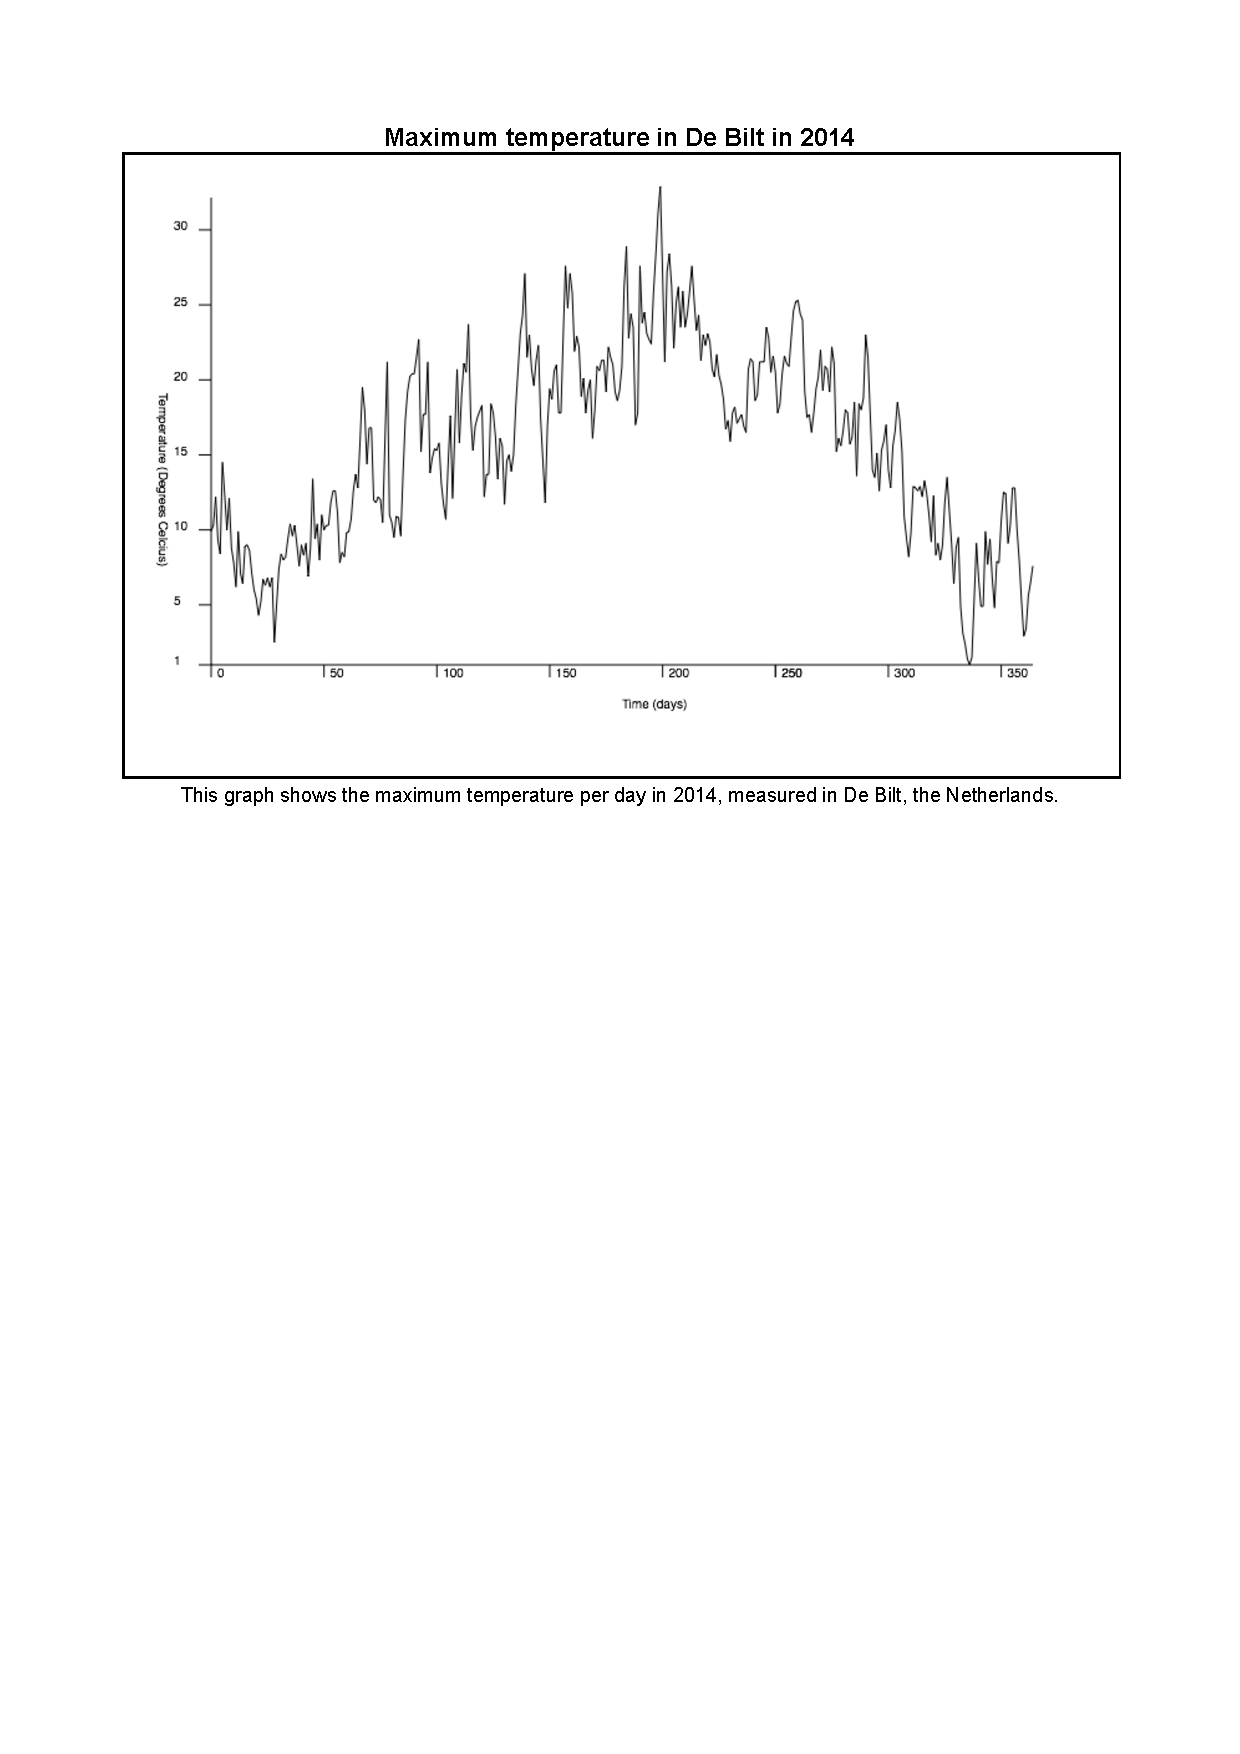
\includegraphics[width=0.7\textwidth]{week4/Graph-Jenny-Hasenack-Cutout.pdf}
\caption{An example temperature graph as created by Jenny Hasenack.}\label{fig:lineplot}
\end{figure}
The HTML 5 canvas element allows JavaScript to draw pictures, the Mozilla
Developer Network has a small tutorial\footnote{
\url{https://developer.mozilla.org/en-US/docs/Web/API/Canvas\_API/Tutorial}}
on the \texttt{canvas}-element that you should read. For this assignment you
will not need to know all the details of the canvas but you should be able 
to at least draw lines, rectangles, circles and text (and how to rotate text).

\subsection{Transforming the data to screen coordinates}
The \texttt{canvas}-element provides its own coordinate system, you will have
to transform you raw data to these coordinates to draw the graph. Figure 
\ref{fig:lineplot} shows you a very simple version of the plot you have to
create for this week. The position encodings for this graph only need linear
transforms, one for the x-axis and one for the y-axis, of the following form:
\[
x_{\mathsf{SCREEN}} = f\left(x_{\mathsf{DATA}}\right) = \alpha \cdot x_{\mathsf{DATA}} + \beta.
\]
Because finding the two constants $\alpha$ and $\beta$ is a bit tedious we 
will create a function that can do it for us. We will use JavaScript's 
support for \emph{closures} to create a function \texttt{createTransform}
that calculates $\alpha$ and $\beta$ and returns a transformation function. The
following snippet of code demonstrates this technique, but you will have to
implement the actual calculation yourself.
\begin{verbatim}
function createTransform(domain, range){
    \\ domain is a two-element array of the domain's bounds
    \\ range is a two-element array of the range's bounds
    \\ implement the actual calculation here
    var alpha = ...;
    var beta = ...;

    return function(x){
        return alpha * x + beta;
    };
}

\\ to use this for instance:
var tranform = createTransform([10, 20], [10, 20]);
console.log(transform(15));  // should log 15
\end{verbatim}
To test this function you can make a transformation that transforms the 
domain $[10, 20]$ to the range $[10, 20]$ and see whether points are
transformed to themselves. This function will work directly on your 
temperature data, but for the dates along the x-axis there is an extra 
complication. An example of a transformation (for either the x or y 
coordinate) is given in Figure \ref{fig:transformation}).

\begin{figure}
\centering
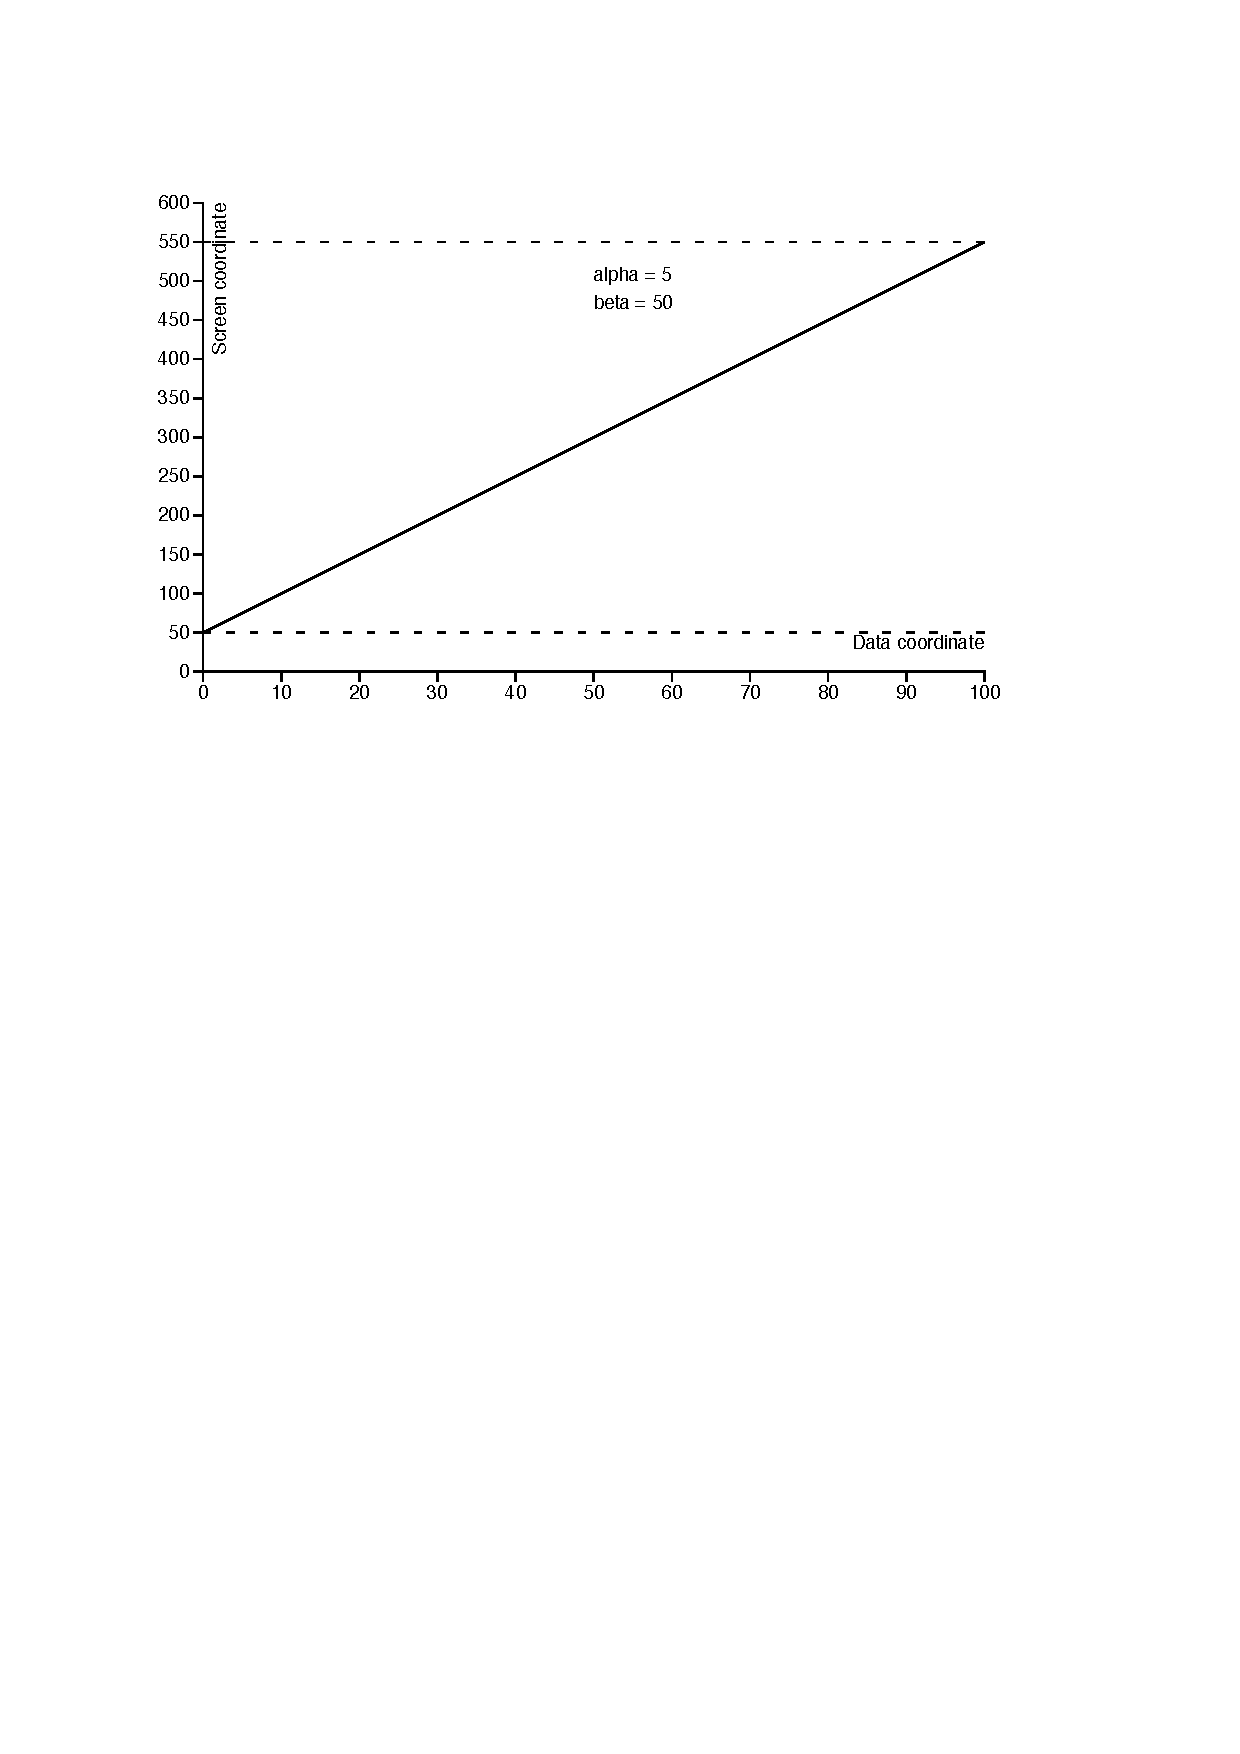
\includegraphics[width=0.7\textwidth]{week4/Transformation-Example-Cutout.pdf}
\caption{An example of a linear transform of the shape $f(x) = \alpha x + \beta$,
that can be used to transform between data coordinates and screen coordinates.}
\label{fig:transformation}
\end{figure}

The x-transform needs to deal with dates, and any calculations involving
calendars tend to get complicated quickly. For this assignment it is ok
to use the \mbox{\texttt{Date.getTime()}} method to change all date
to milliseconds since January 1$^\mathrm{st}$ 1970. These milliseconds can
then be transformed into days since the start of your data (so the x-axis
would run from 1 through 365 or 366 days depending on the year you chose).

\section{Extra credit}
\begin{itemize}
    \item Create an x-axis that uses calendar dates (in stead of days since
          the first date in the data set.
    \item Loading the data from file (you will need \texttt{XMLHTTPRequest}).
    \item Nice graphical presentation will be credited.
\end{itemize}


\subsection{Checks before submitting}
\begin{itemize}
    \item See Chapter \ref{chapter:submissions} for general guidelines that
          submissions need to follow.
    \item Does your submission contain a PDF with the answers to the 
          questions in Section \ref{section:js-questions-1}, and the complete
          implementation of the temperature graph?
\end{itemize}
